\documentclass{sig-alternate}
%\usepackage{algorithm}
%\usepackage{algorithmic}
\usepackage{url}
\usepackage{subfigure}

\pdfpagewidth 8.5in
\pdfpageheight 11in

\title{Crowdy: Social Crowd Visualization}

\numberofauthors{1} 
\author{
    \alignauthor Jeffrey McGee, Zhiyuan Cheng, Chiao-Fang Hsu, Pratheek
    Kumar Akireddy \\
    \affaddr{Department of Computer Science and Engineering, Texas A\&M
    University} \\
    \affaddr{ College Station, TX 77845 USA} \\
    \email{jeffamcgee@gmail.com, zcheng@cse.tamu.edu, drakihsu@cse.tamu.edu,
    pka293@cse.tamu.edu}
} 
\begin{document}

\maketitle
\begin{abstract}
Microblogging systems have provided society with a more transparent channel
for information distribution. Each individual is empowered to spread news
and build their social network. With the freedom of information generation,
the issue now is identifying, organizing, and visualizing useful information.
For this project, we want to design an user interface that takes
both usefulness and usability into consideration. Our system will
adapt to different types of users and display the crowds that form in a specific
period of time as well as the topics discussed by the crowd from Twitter. The
interface should both optimize the user experience and system speed. For
evaluation, we will design a user study to
test the efficiency, effectiveness, and satisfaction of this system to our
potential users.
\end{abstract}

\category{H.5.1}{Information Interfaces and Presentation}{Multimedia
Information Systems}[video]
\category{H.5.3}{Group and Organization Interfaces}[collaborative computing,
computer-supported cooperative work]
\category{H.5.4}{Hypertext/Hypermedia}[architecture]

\terms{Design, Experimentation, Human Factors}

\keywords{interface, crowd, Twitter}

\section{Introduction}
Along with the rise of real-time social web, the power of information
distribution is no longer limited to the small set of news media but the
massive amount of ordinary individuals. Websites like Digg and Reddit provide
a news aggregation platform that filter and display interesting news pieces
recommended by other users; social media object sharing sites like Youtube and
Flickr let users upload and browse videos and images; microblogging systems,
like Twitter and Buzz, enable every user to host a broadcasting station of
their own; last but not least, Facebook allows users to build their own
social network and share their everyday experience with their friends.
Thus, there is a demand for services that
exploit these massive sources of data. People are looking for a new
generation of applications for monitoring, analyzing, and distilling
information from the prospective web of real-time content that reflects the
current activity of the web's participants. The shift toward fresh web content
can be seen in the growing interest in mining large-scale social media for
information discovery and brand management, for intelligence analysis by the
government and state media, and in identifying and disseminating disaster and
emergency-related information.

Comparing with the traditional web information applications that apply
expensive off-line analysis of web data, the new generation of real-time web
applications must be able to consume, process and display the massive amounts
of data on-the-fly. In this project, we look particular into Twitter, a
microblogging platform. We want to provide users a manageable
exploratory interface that displays the crowds and their associated
participants/content at each time period.  We define a ``crowd'' to be a
potentially short-lived ad-hoc collection of users.  There are several ways to
identify crowds: users who message each other, users who are nearby, and users
who use similar terms. In Twitter, there are potentially 100s of millions of
active users inserting new messages into the system at a high rate. With
existing algorithm and architecture built by our lab in the backend, our goal
is to reveal the ad-hoc crowds of users that reflect the real-time interests
and highly-temporal group affiliations in a clear and manageable fashion.

Even though our current data is from Twitter, we expect the system to be useful
to users who are not familiar with Twitter. In fact, our system can be of
useful to several types of users with different purpose in mind.

\subsubsection{How Might We Help}
Apart from the original Twitter interface that provides only a local view of
the most current tweets issued by each user's friends or some local trending
topics, our final system should be able to aggregate the data to find global,
regional, and local phenomenons. The final product is also adjustable that fit
into different expertise and purpose of usage based on the role of the users.

\subsection{Conceptual Model}
The conceptual model of our system is a tool for finding patterns, trends, and
communities. The interface displays groups of people who are talking with each
other, puts their conversation on a map, and finds important words in the
conversation. Users will expect different types of filtering options such as
filtering by area(geo-feature), by time(timeline snapshot), by
keyword(free-text, hashtag) or by the expecting property of the crowds(the
longest living crowd, the most engaging crowd). The default view of the system
is a set of global crowds discovered recently.


\subsection{User}
To better design our system interface, we want to understand our potential
users. For different kinds of users, there exhibits different patterns of
properties like the frequency of usage, the level of experience, the behavior
tendency and the tuning options availability.
\begin{itemize}
    \item Analyst: Government or media analyst are experts in information
    trending and market research. They use the system regularly with the
    frequency between once per day to once per month depending on the urgency
    of the monitoring task itself. They would like to have a customized interface
    that is able to apply a variety of filters on the fly. While they are 
    investigating the data using our system, they are likely to be writing a
    report.

    \item Twitter Users: Twitter users who already have familiarity with the
    Twitter world can use our system to learn about crowds
    and hot-topics. The may use it regularly or occasionally. They adopt our
    system to assist their twittering experience. They might not devote a large
    amount of time and effort but just want a quick and fresh view of the
    current trend. For this purpose, we should provide a simple and
    personalized content display with some easy filtering options.

    \item Regular People: regular users with no Twitter experience will use
    our system as a window to gain an idea of what is currently happening
    in the Twitter world. To satisfy their curiosity without personalized
    history to learn from, we provide a global trend as the first look.
    Ideally, the users will come back and build a history profile so we can
    customize the display in a long run. people could use it just once or, if
    they like the system, several times per day.

    \item Business People - corporate employees are particularly interested in
    their own product or company. Like the analysts, they are asked to perform
    the trending survey in a regular basis. They are trained in finding
    information related to their product. They use our system to find the
    opinion from the general users. They also study their competitors in a hope
    to improve their own. For this type of user, we can do highly customized
    interface to pre-filter the crowds to display. We may also prepare a set of
    templates so the business people with no computer science knowledge can
    easily drag-and-drop views related to their competitors and their own
    business side by side.

\end{itemize}

\subsection{Cognitive Issue}
Some cognitive issues we need to consider include the other activities our
users might be engaging in simultaneously. For example, the Twitter user might
be browsing Twitter and plan to use our system to understand the crowds that
talk about a certain keyword of interest. Another situation can be finding some
interesting topics while playing with our system and decide to do search to
read the related news article from Google or NY Times. Or, our users may
discover an exciting crowd/topic and eager to share this discovery to his
friends on the social websites(Twitter, Facebook, etc). That is to say, we does
not expect our user to keep 100\% focus on interacting with the system. We need
to provide mechanisms for tip reminding of behavior history. 

In addition, with the nature of the temporal massive data, we do not expect our
users to remember where to find the crowd/topic of interest that the user just
encountered. We want to provide a Workspace panel so to release the stress on
the memory requirement from the user.

\section{Related Work}
Twitter\footnote{http://www.twitter.com} is a microblogging platform which is
fast gaining popularity\cite{Oreilly:2009} among broad sections of society and
has a global outreach spreading from developed, urban nations like the United
States where it has a high adoption rate \cite{Java:2007}, to developing
countries in parts of Asia and South America.

Along with working on understanding microblogging usage and communities
\cite{Java:2007}, the main author - Akshay Java was one of the first few who
dealt with the measurement of the usage and nature of communities in
microblogging. In his latter study \cite{Java:2008}, he presented his
observations of the microblogging phenomena and user intentions by studying the
content, topological and geographical properties of such communities. He found
that microblogging provides users with a more immediate form of communication
to talk about their daily activities and to seek or share information.

When it comes to visualization of the social crowd, a tool which in some ways
shows similar objectives as us and stands out among the rest is Vizster
\cite{Heer:2005}. It is a visualization system for which can be used for
exploration and navigation of the social networks of any scale. The system
provides facilities to improve the functionalities like discovering people or
connections which can help in promoting awareness of community structure and
exposure to information. It maintains a fun element to it while providing these
given features. It was aimed to provide specific end-users, functionalities
like situated exploration and visual analysis of big-scale communities. It is
based on a design of network layouts which have features like supporting visual
search and analysis, exploring connectivity in large graphs and automatic
identification and visualization of structures of communities.

Another related study was on how web-based retrieval from twitter can be used
as knowledge base \cite{Cheong:2009} which shows that the visualization system
we try to attempt can be helpful. Marc Cheong et al. in this study tried to
analyze demographics of the Twitter users and attempted to provide and analyze
the trend in Twitter into what's going on in the real world. They enabled us to
understand the underlying characteristics behind the trend setting in Twitter
and thereby providing a new perspective on the contributors of a trend. They
used visualization techniques along with artificial intelligence-based data
mining methods to classify the Twitter messages dealing with the trend topic.

Identifying highly dynamic ad-hoc collections of users what we refer to as
crowds in massive social messaging systems like Twitter and Facebook is
important \cite{krishna:2010}. Kamath et al. in the study suggest an
efficient locality-based clustering approach for identifying crowds of users in
near real-time compared to more heavyweight static clustering algorithm. The
study consisted of 711,612 users and 61.3 million messages, and tells what
approaches to follow to efficiently and effectively identify Twitter-based
crowds.

In the other study based on the previous one, Kamath et al
\cite{krishna:2011}, they add another salient feature - a novel crowd tracking
and evolution approach for linking crowds across time periods. Unlike the more
static and long-lived group-based membership offered on many social networks
their goal was to support the discovery of organic and highly-temporal group
affiliation, which they refer to as ``transient crowds''. A transient crowd
according to them is a potentially short-lived ad-hoc collection of users bound
together by some common thread - which can be communication-based,
location-based or interest based. We are inspired by this idea of formation and
detection of crowds. We try to implement detection of crowd in Crowdy in a
similar fashion.

Some other studies related come from areas like social network visualization,
short text visualization, progressive disclosure, and user modeling. Considering
social network visualization , studies like \cite{Boyd:2008} by Boyd et al described features
of on-line social networking sites and the history of the social networking sites,
and the changes during their developments.Deeper understanding of the social
networks can help boost the research in social network visualization. In Moreno's
following work \cite{Moreno:1953}, he emphasized the use of pictorial representations to map
social relations and the embedded patterns. He considered people as nodes in the
network and relations between people as the edges in the network.Laumann et al
\cite{Laumann:1966} applied computational procedure, multidimensional scaling to locate nodes in
visualizing network. The authors are also the first to plot the networks in three
dimensions. Other examples of good visualizations can be Facebook Friend Wheel
\cite{facebook_wheel} which visualizes a Facebook user's network of friends in a wheel format and
Trendsmap \cite{trends_map} which plots real time trending topics over two-dimensional (latitude,
longitude) world map, and you can zoom in to see the trending topics for a specific
location or an area. 

In the area of short text visualization, studies like \cite{Bishop:2007} tell that these social
web-sites serve to fulfill their users' desires to interact with and help others.
The authors also proposed a 3-level framework for understanding why members of online
communities participate or not. According to the 3-level framework, users make
comments or short-text post to have their voice be heard. Leggett and Shipman \cite{Leggett:04} 
proposed and described the characteristic of interactive communication in seven
dimensions in a similar way to examine characteristics of communication for a
commenting system like roles,voices,interaction,indirection,history,narrative
and media. In \cite{Hsu:09}, they tried to understand how an on-line community itself
perceives the relative quality of its own user-contributed content and further
used the information to promote valuable opinion from the flood of comments
that attached to each social object.We compared three different visualization
approaches including the traditional list view, the quantitative aggregation
view and the personalized space view. We learned that, to best present massive
metadata such as user contributed comments to the end user, a personalized
filtering model is needed and that a 2D space positional layout is desired
such as in the case of Plurk and Opinion Space systems.

In the area of progressive disclosure, Phan et al built a prototype of a system
that visualized packet traces from a computer network \cite{Phan:07} which is similar to
the problem investigated. They introduced the concept of progressive multiples
which combines progressive disclosure with small multiples. In Scalability in
System Management GUIs \cite{Dieberger:06}, the authors use semantic zooming to show information
about network configuration at various levels of detail, which can tell about
the way progressive disclosure can be used for system administrators.In An
Interactive Ambient Visualization for Code Smells \cite{Murphy:10}, the authors describe a
method for alerting uses about code that may need refactoring. They created a
plug-in for Eclipse that detected questionable code and alerts the programmer.
This shows progressive disclosure for software developers.

Involving user models and visualization into the picture, studies like \cite{Schlungbaum:97} tell
that the individualization often depends on the user's expectation of the user
interface which might be adapted or adaptable or adaptive user interface. Papers
like \cite{Ho:01} explain that the user model selection is crucial for any tool and how
the visualization can help in the discovering and building knowledge. Data and
knowledge visualization module of such a system can be used to help the user
interaction in other modules. This helps in better user interaction experience
irrespective of which module of the system he/she is interacting with.The user's
knowledge, preferences, goals etc. are generally included in the user model when
visualization is concerned in such tools \cite{Henderson}. Also, critical factors like cognitive
load on the user ought to be considered when such tools are made to ensure
effectiveness.The identification of target users is also a important factor to be
considered.Model-based tools like TADEUS can include explicit task and user models
in their system, over potential to work in integrated user interface development
environments and support the entire user interface life cycle. Although research
papers like \cite{Schlungbaum:97}, talk about how different software tools can be used for helping
the user designers create interfaces with consideration of user models , there have
been efforts to combine user model with task and domain models to help developers
in creating and designing user interface \cite{Tran:10}. Systems like DB-USE along with TADEUS
help us in understanding of how user model can be combined with other models to help
in creating/designing better user interface for applications which are mainly
concerned with visualization.

\section{Interface Design}

This section illustrate an outline of the prototype. We want to provide
the user with a simple and flexible interface to maximize their options for
exploring while minimizing their memory overhead. Existing web applications
show that the most general task should be the main focus and the other
available options may be placed on the side or hidden according to their
frequency of usage. Since the primary function of our system is to visualize
the Crowds emerged over time, the crowd display window is our
first priority. In the crowd display window, we
consider the needs of personalization for our potential users(e.g. Analyst).
There is a global view panel and a personal workspace panel. The personal
workspace panel distinguishes from the global view panel in a way that it only
shows the set of crowds marked by the user when exploring in the global view
panel. Inside each view, we need to decide the best format to condense
a massive amount of data. Each crowd has metadata associated with it such as
starting and ending time, crowd participants, topics, tweets,
location data, etc. To effectively organize these properties to assist quick
and convenient retrieval by the user, we consider these two formats: timeline
and list. For both view panels, these two formats are included but sized
unequally. The size is adjustable(in the option panel) according to the user's
need. Generally, ``timeline'' is more suitable for overview a large number of
crowds while ``list'' is better for investigating details in a smaller set of crowds. We
also provide several filtering options for both timeline and list format in the
option panel. Some detailed components in these three panels are listed below.

\begin{itemize}
				\item Timeline format displays the evolution of each crowd.
        First of all, a crowd is shown as a line from the starting time
        to the ending time. The size of the participants over time is
        indicated by color(e.g., small-large-medium $\longrightarrow$
        green-red-blue). The top three keywords that describe the topic of
        the crowd are displayed explicitly on the timeline along with
        the crowd line. Extra information about the crowd can be viewed
        in the pop up box when the user clicks on the crowd line.
        
        \item List format displays each crowd with some specific
        sorting order. The default sorting order is by the starting
        time. Some other available sorting functions include the
        ending time, the size of crowds and the ranging time. In the
        list format, crowds are displayed explicitly in three columns:
        time period, participants and size of the crowds. If the crowd is clicked, it will show the list
        of tweets and other detailed information in a slide down window
        form.
%    \item \textit{Global View Panel} : The global view shows the global crowds
%    in different format. When a crowded is marked by the user, a flag will be
%    placed in front of each crowd item in each format.
%
%    \begin{itemize}
%        \item Timeline format displays the evolution of each crowd.
%        First of all, a crowd is shown as a line from the starting time
%        to the ending time. The size of the participants over time is
%        indicated by color(e.g., small-large-medium $\longrightarrow$
%        green-red-blue). The top three keywords that describe the topic of
%        the crowd are displayed explicitly on the timeline along with
%        the crowd line. Extra information about the crowd can be viewed
%        in the pop up box when the user clicks on the crowd line.
%        \item List format displays each crowd with some specific
%        sorting order. The default sorting order is by the starting
%        time. Some other available sorting functions include the
%        ending time, the size of crowds and the ranging time. In the
%        list format, crowds are displayed explicitly in three columns:
%        time period, participants and size of the crowds. If the crowd is clicked, it will show the list
%        of tweets and other detailed information in a slide down window
%        form.
%    \end{itemize}
%
%    \item \textit{Personal Workspace Panel} : Similar as the Global View Panel
%    but with only the set of crowds marked by the user in the Global View
%    Panel.
%    \item \textit{Filter Option Panel} : This panel explicitly displays a set of
%    the most frequently used filtering options such as search and timeline scaling.
%    We also provide the user with flexibility to adjust the default
%    settings we provided such as the primary display format in the View
%    Panel, list sorting function and time period filtering. Other filtering
%    options are hidden and can be expanded with a click on the right bottom corner
%    of the Panel.
\end{itemize}

\section{Implementation}

\subsection{Workflows}

The system is designed to run in a user's web browser. As a result, we decided
to use some fairly standard web tools to implement the system. The system that
we are building the user interface on top of exposes a RESTful API. Although
it is not a part of this project, it is important to understand how the backend
works, and how it fits into this project. The work flows of the system can be
decomposed into following parts: (i) a crawler retrieves tweets from Twitter using
Twitter's REST API, search API, and streaming API; (ii) the corresponding data
go through several filters that add additional information to the users and
tweets; (iii) a program finds groups of users (i.e., crowds) based on their 
communication patterns; (iv) the data of crowds are stored as JSON in a MongoDB
database; (v) the backend also provides the RESTful API that we connect to; (vi)
to retrieve data, our system makes an HTTP GET request to the server, and the 
server returns data in the JSON format, which is easy to decode in Javascript.
To make the architecture clean, we never allow our GUI directly read from or 
write to the database.

\subsection{Techniques}

We are writing the portion of our web application that runs on the server in
Python, since that is what our team has the most experience with. We chose the
CherryPy framework to build the application because it is simple and lets us
write modular, testable code. We are using the Jinja templating engine to
generate the HTML pages. This makes it easy to have a consistent look across
all of our pages without duplicating code.

The code that will run on the user's web browser has to be written in
Javascript. We use the jQuery library to handle events, retrieve JSON, and
abstract away the idiosyncrasies of the various web browsers. We are using the
Simile Timeline library \cite{simile} to produce the crowd timelines. In the 
future, we may use the Google Maps API to display crowds on a map.

\subsection{Features}

In the system, we provide three perspectives to visualize the crowds: (i) timeline;
(ii) list; (iii) map. We also support search function so users are able to search 
crowds given query of text, time period of crowd, and size of crowd, and visualize
the crowds with the three options of perspectives.

\subsubsection{Timeline}

\begin{figure}
\centering
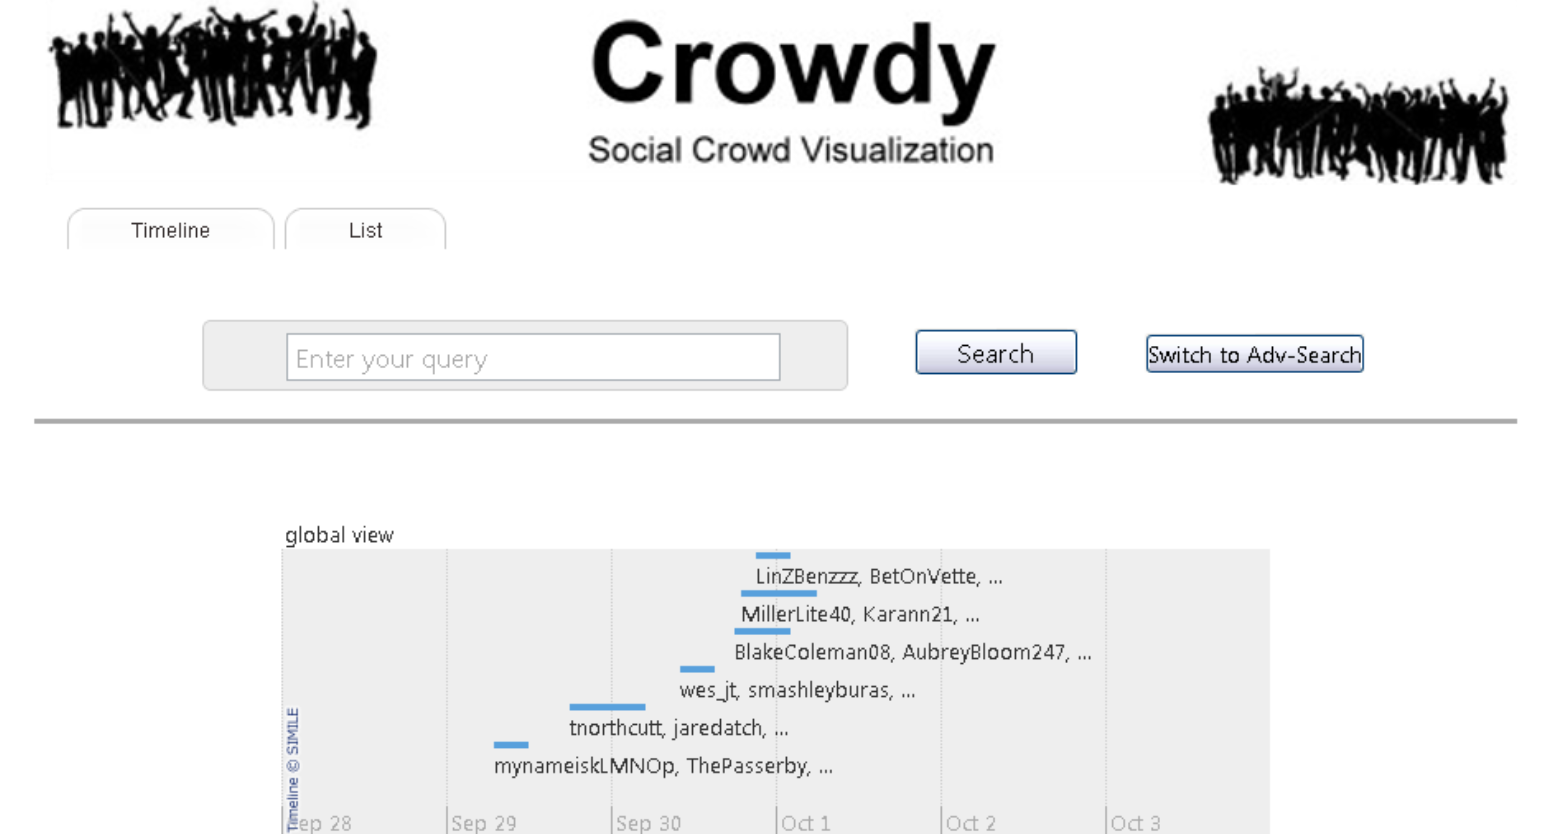
\includegraphics[width=\linewidth]{imgs/TimeLineView.png}
\caption{Timeline View}
\label{fig:TimelineView}
\end{figure}

\begin{figure}
\centering
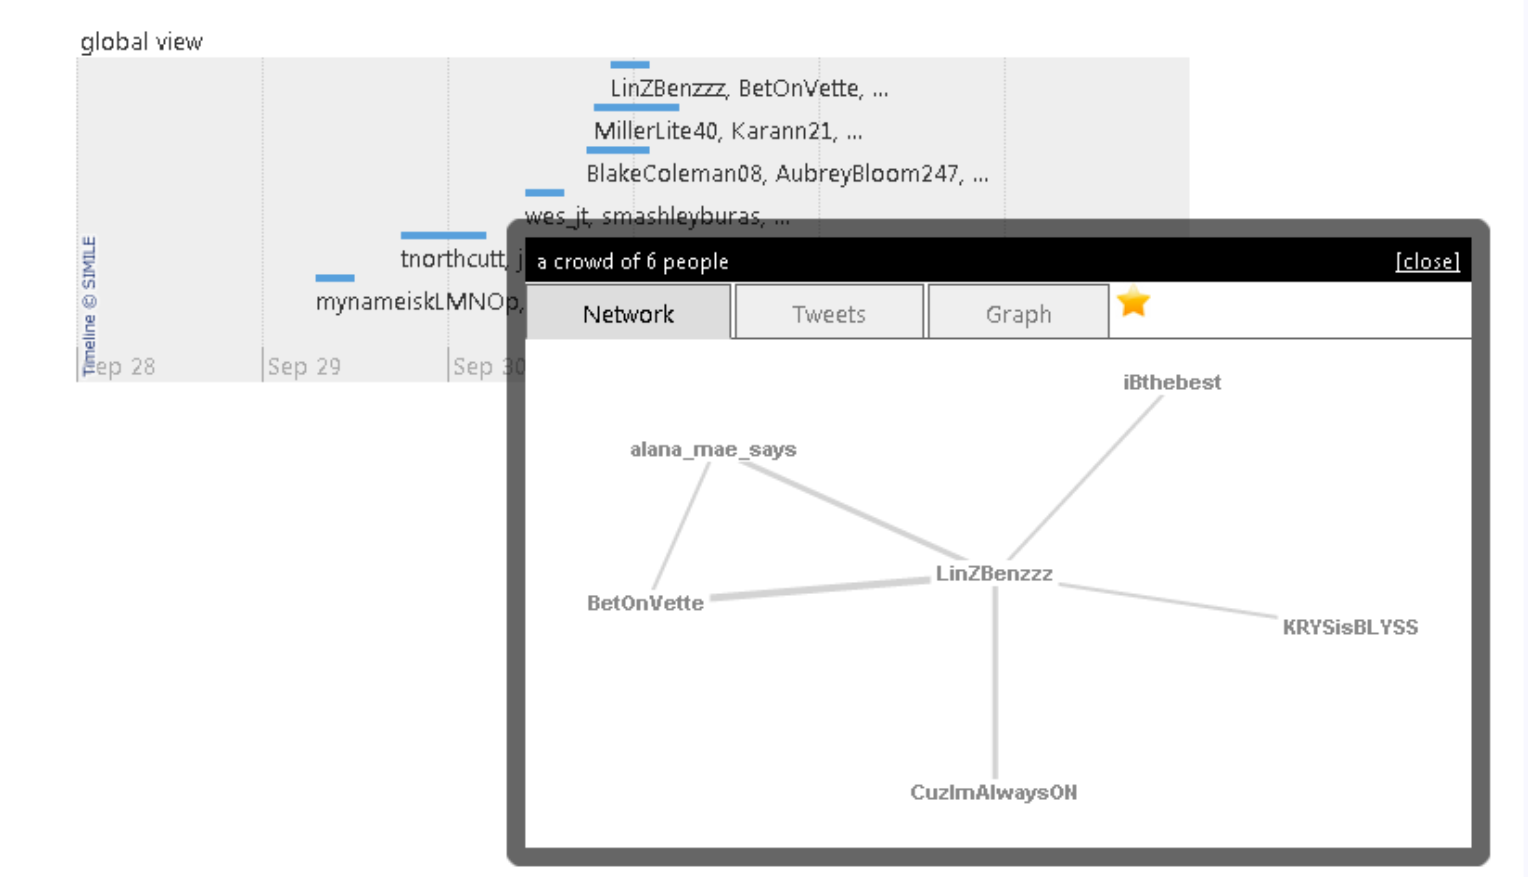
\includegraphics[width=\linewidth]{imgs/CrowdViewInTimeLine.png}
\caption{Crowd View In Timeline}
\label{fig:CrowdViewInTimeline}
\end{figure}

We apply the Simile Timeline library which is developed by MIT's Computer
Science and Artificial Intelligence Laboratory. The timeline as shown in figure \ref{fig:TimelineView} shows all of the
crowds at a given time span.  The timeline allows the analyst to zoom in on a
specific time, and move forward and backward thorough time.  The visualization
shows how long the crowd lasts, and the size of the crowd. We may make the
crowd taller or shorter based on the size of the crowd.  We will also display a
few keywords from each crowd. After a crowd in the timeline is clicked, a pop up ``Crowd View'' window will show the detailed information of this particular crowd (Figure \ref{fig:CrowdViewInTimeline}).

\subsubsection{List}

\begin{figure}
\centering
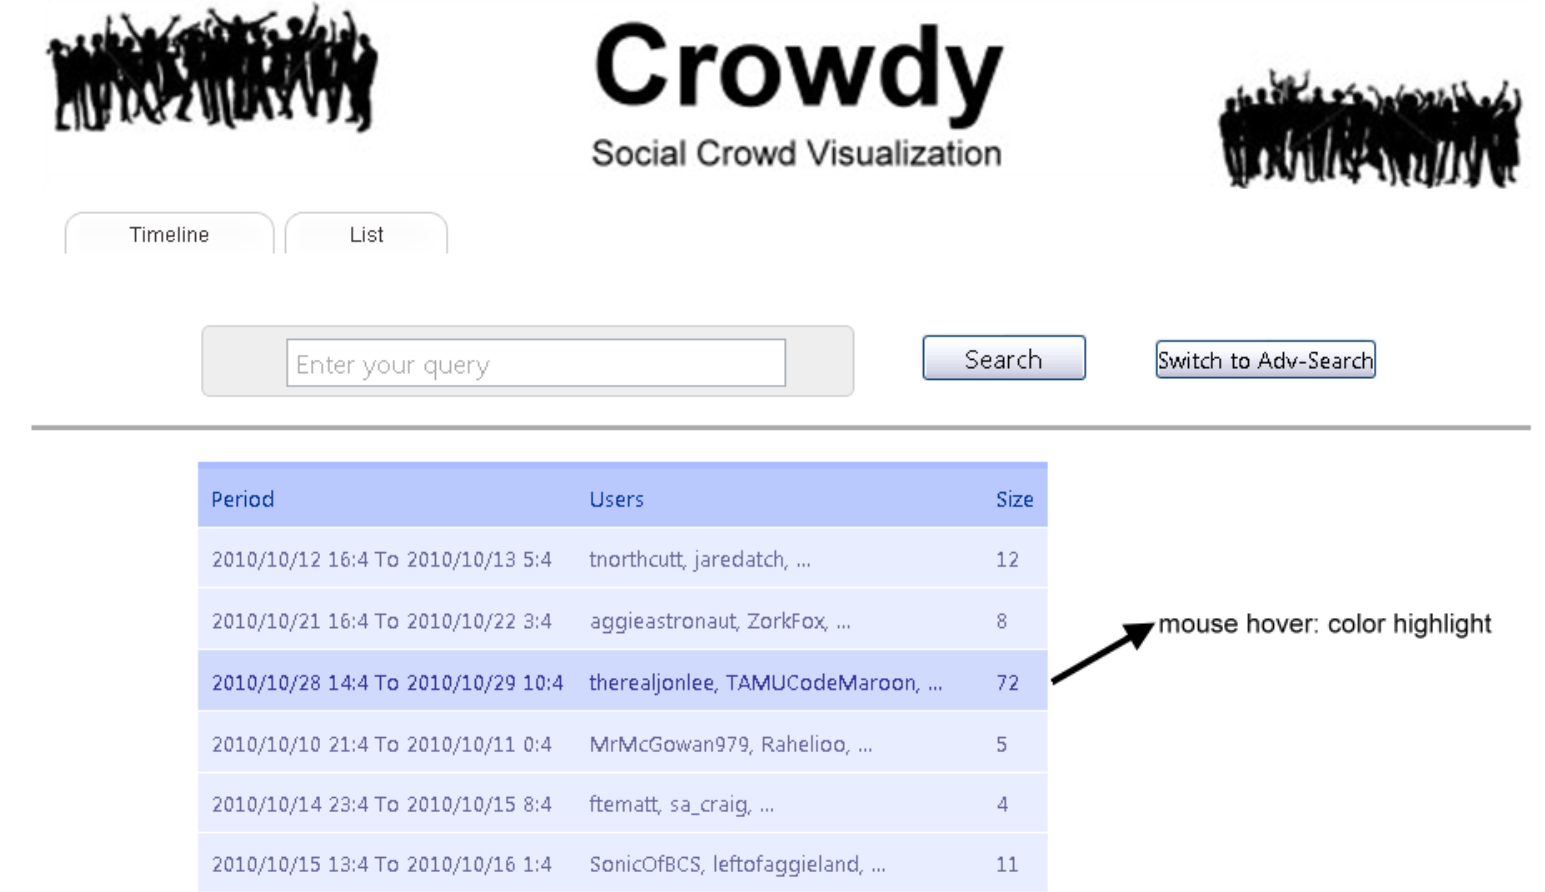
\includegraphics[width=\linewidth]{imgs/ListView.png}
\caption{Overall List View}
\label{fig:ListView}
\end{figure}

The list view as shown in Figure \ref{fig:ListView} requires a dynamic table in
which it displays as many rows as the amount of crowds returned by the API.
Concretely, we issue an HTTP request to get the crowds in the database in a
JSON object. The Javascript creates the dynamic table which includes the
following columns: Period, Users and size of the crowd. We pick the screen
names of two users with the highest degree centrality to represent the crowd.
Once the row that represents a crowd is
clicked, a slide down box with detail information(crowd user network, tweets)
will be shown below. There are three types of information available for users
to choose from: Network, Tweets and Graph and a ``star'' mark. 

Each crowd has a star-feature attached to it which can be used by the user to
mark his favorite crowds. This feature is present in the detailed view of the
crowd which is activated as said earlier by selecting the row of a crowd. This
is used to rearrange the list of crowds with the starred crowds appearing at
the top whenever the user comes back to the list view. The user can mark any
crowd as starred or unstar the ones that are already starred at any point of
time. 

\subsubsection{Search}

\begin{figure}
\centering
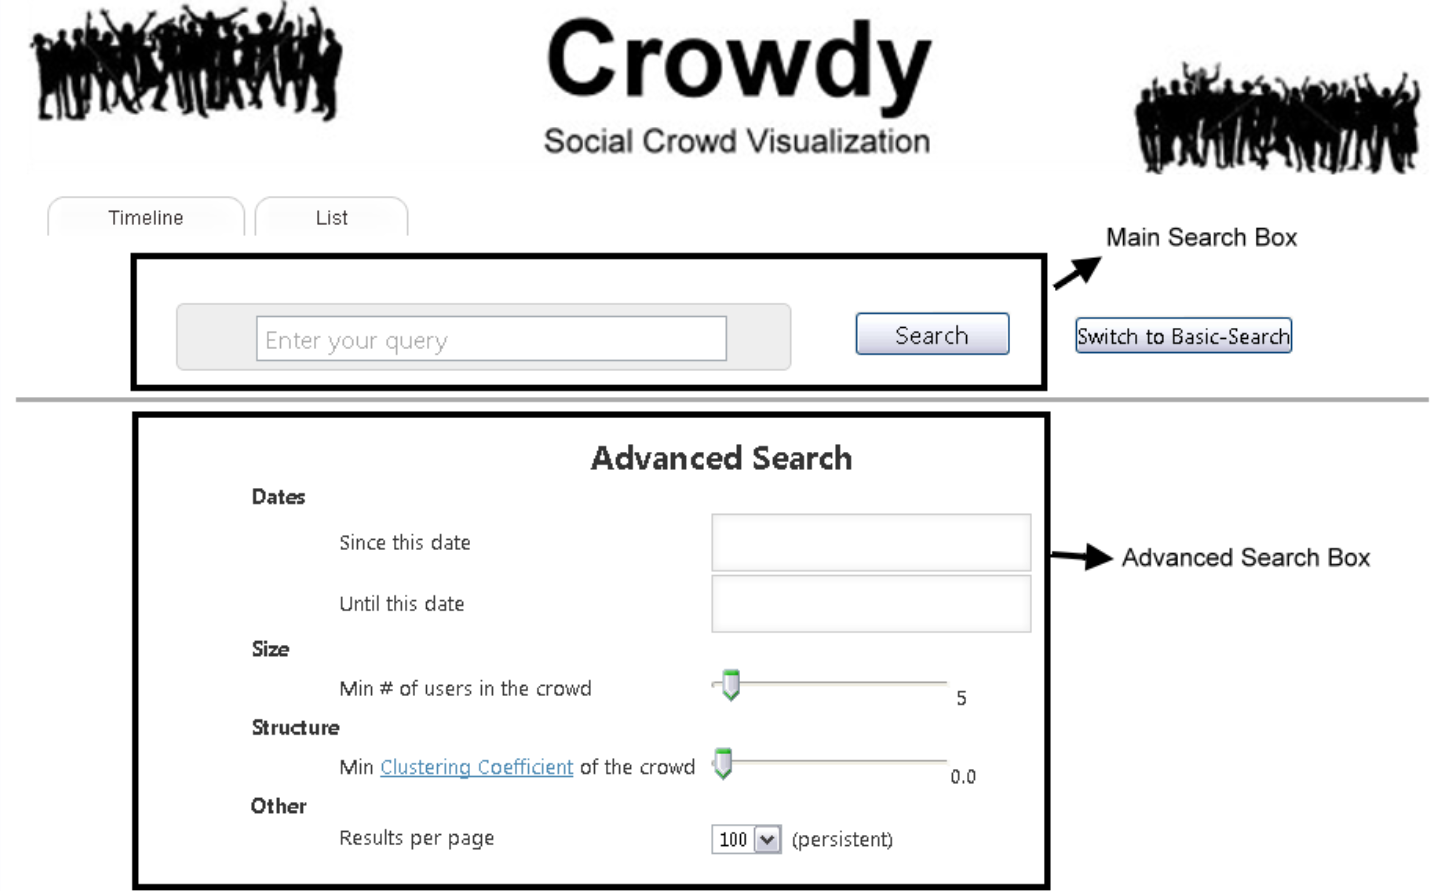
\includegraphics[width=\linewidth]{imgs/Search.png}
\caption{Search}
\label{fig:Search}
\end{figure}
In the search function of the system, we provide a main search box in which 
users can type a textual query to search for crowds which contains the query.
Besides, users can also click the link of advanced search, so that they can 
choose options of words, time period of crowd, size of crowd, value of clustering coefficient of crowds,
and results they would like to see per page. The layout is shown in figure \ref{fig:Search}. We maintain indices for each kind
of queries in the MongoDB database, so that we can efficiently return the results
to users. Whenever a query is issued, the systems send a HTTP GET request to the
backend, and the server would return the corresponding search results.

In our future direction, we will also provide query options like location, user's
screen name, . So that users can search crowds that are in a specific city or an 
area, and also search crowds that a specific user is involved in.

\subsubsection{Crowd View}

\begin{figure}
\centering
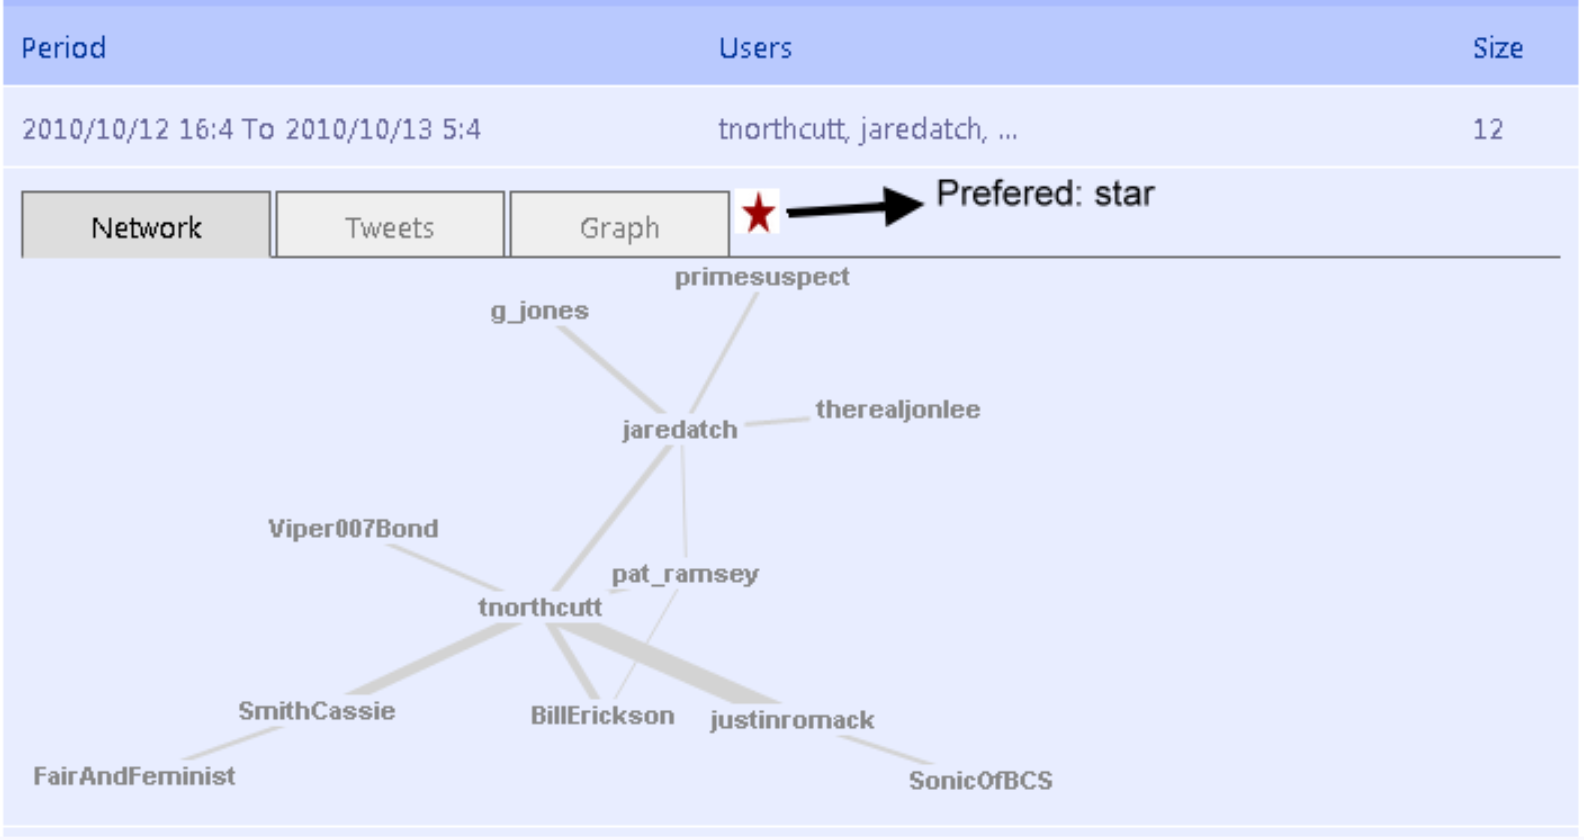
\includegraphics[width=\linewidth]{imgs/NetworkInList.png}
\caption{Network View in List}
\label{fig:NetworkInList}
\end{figure}

\begin{figure}
\centering
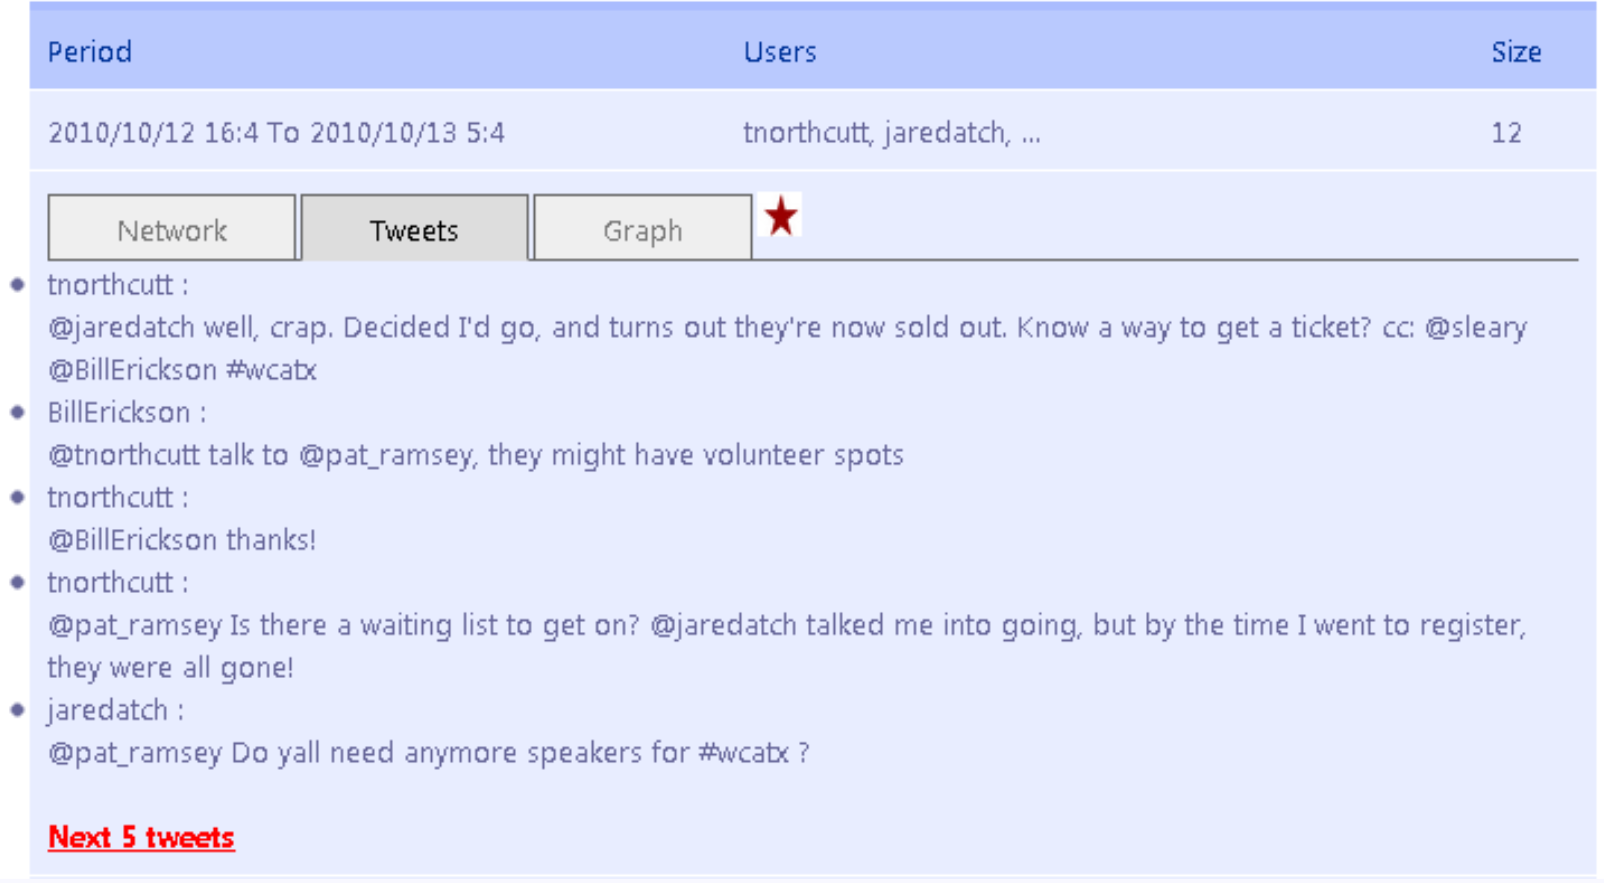
\includegraphics[width=\linewidth]{imgs/TweetsInList.png}
\caption{Tweets View in List}
\label{fig:TweetInList}
\end{figure}

\begin{figure}
\centering
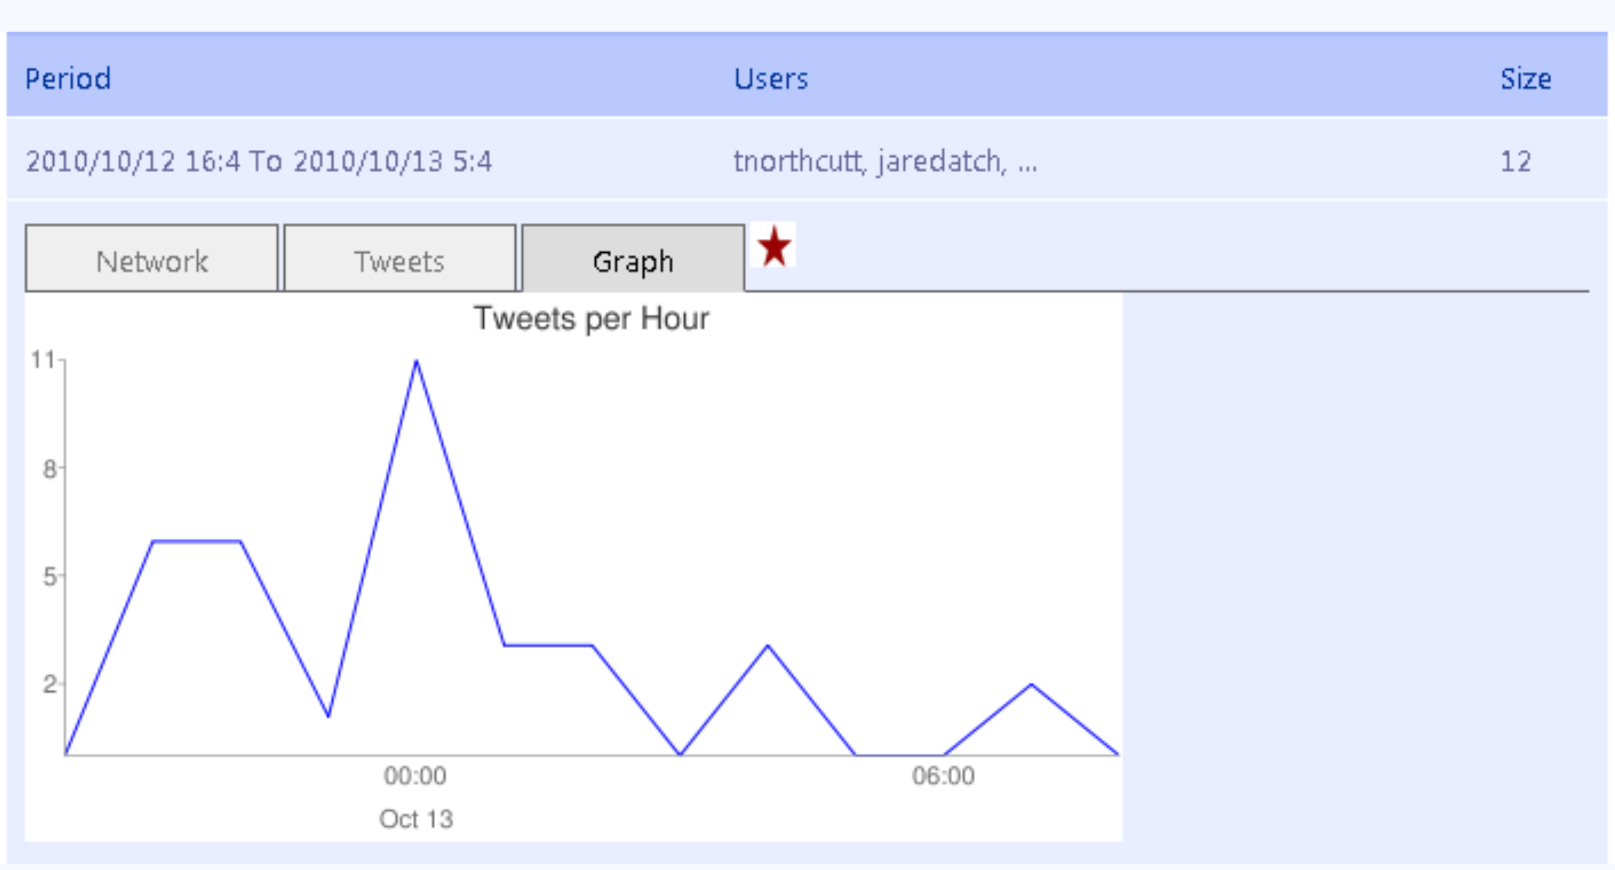
\includegraphics[width=\linewidth]{imgs/GraphInList.png}
\caption{Graph View in List}
\label{fig:GraphInList}
\end{figure}
When an analyst clicks a crowd in the list, timeline, or map view, we show an
expanded view of the crowd. This is a form of progressive disclosure, where we
give the analyst more information as they need it.  

The default view is the Network information as shown in figure
\ref{fig:NetworkInList} where nodes represent users, and edges represent the
tweets. The network graph show the relationship of the users involved in this
particular crowd based on the tweets mentioning activities. A thicker edge
between two users indicates more tweets sent between that pair of users. In the
future work section of this paper, we discuss ways that this could be improved
to let the user drill down even more.

In the Tweets tab we can see a set of tweets in this crowd like in figure
\ref{fig:TweetInList}. In order to provide users a cleaner page view, we
restrict 5 tweets per page to show in the slide down box and thus, a multiple
page navigation is possible. Users can click on the ``Next 5 tweets'' if it is
available.

The Graph view shows the activeness of the crowds in an hourly time basis.
Figure \ref{fig:GraphInList} gives a crowd graph example. We can see how a
crowd start to engage, develop and die over time.


\section{Evaluation Plan}
In order to evaluate our system, we plan to conduct a 2-step usability study
which includes a pilot study, and an evaluation study. In the pilot study, we
will ask a relative small number of users (e.g., 5 - 10 people) to try our
system, and fill in the usability questionnaire. Then, we will refine the system
based on the feedback from the pilot study (i.e., fixing bugs reported by users,
modifying features that were not preferred). Finally, a large scale evaluation
study also in the form of questionnaire will be conducted on a user base of 30 -
50 users including three types of users we mentioned earlier: normal users, 
Twitter users, and analysts. The refinement step and the large-scale detailed
evaluation study will be generated after the step of the pilot study. Thus, in
this report, we only focus on the design of the pilot study.

\subsection{Pilot Study}

The pilot study we propose consists of two parts. First, we will ask the users
to use our system to find several conversations that they find interesting.
Next, we will use a questionnaire to gather basic demographic information and
answers to seven questions with a five point Likert scale (i.e., strongly
agree, agree neutral, disagree, and strongly disagree) and four open questions.
The Likert scale questions are listed below:

\begin{itemize}
\item The interface for timeline view is easy to use.
\item The interface for list view is easy to use.
\item The search feature for timeline view is easy to use.
\item The search feature for list view is easy to use.
\item I could use the search features to find crowds that I was interested in.
\item The star feature helped me organize crowds.
\item When I star a crowd, all the crowds on the page should be re-arranged in real time to place the starred crowd on top.
\end{itemize}

We would also ask some open-ended questions:
\begin{itemize}
\item What are the features that you like most? Why?
\item What are the features that you don't like / hate most? Why?
\item What features that you would like Crowdy to implement in the future?
\item Do you have any other comments? 
\end{itemize}

Once we have the results of the pilot study, we can refine the test procedures
and questionnaire. We will run this study on a larger group of people.

\section{CONCLUSIONS}
In conclusion, we have implemented the Social Crowd Visualization system as a
web application that enable users to visualize,summarize and organize temporal
crowd formation on Twitter. We studied several types of potential users and
design the interface carefully to meet their needs. We implemented a few
different layout format and a search component to ease the crowd retrieval
effort on user. Finally, we design a sequence of possible evaluations for this
system. The interface will be continually improved as it is also an on-going
DARPA project with the InfoLab. 

\section{FUTURE WORK}
There are several natural extensions of this system that we will carry on in the near future. Fist of all, we see that building user model may be beneficial to enhance the user experience over different operation sessions. Currently, the user behaviors are recorded globally as if there is only one user using Crowdy. Once the user model component is implemented, we can separate individual preference and possibly show the preference of users with different level granularity. In addition, we can better learn the user preference as different role and improve our data filtering mechanism accordingly.  

Secondly, we will also consider implementing map view. The map view can better present the geographical aspect of the crowds. As a portion of the tweet data we have crawled contains location information, it would be interesting to show as a map how users in a crowd distribute.

In third, we see a need to contextually summarize the crowds. With informative keywords to represent each crowd, we can obtain more valuable search results. For example, the search of ``howdy'' should be some crowds with ``howdy'' as the main theme instead of a big crowd with ``howdy'' appears in 1 tweet only. Besides, users of the system will be able to distinguish and identify crowds of interest at a first glance. This can ease the browsing experience of users.

Fourth, we can make the network view more interactive. For example, when the
analyst clicks on a node, we can give the analyst more information about the
Twitter user that was clicked on. When the analyst clicks on an edge, we can show the
conversation between those two users.

Finally, we want to improve the timeline component so it can support zoom in and zoom out functionality for better scaling flexibility. For example, crowds within the same day are grouped in the default view. The users might want to zoom in and see a hourly-display of crowds in each day or zoom out to browse crowds in each of the 12 months of a year.

\bibliographystyle{abbrv}
\bibliography{reference} 
\end{document}
